\section{Evaluation of the modelled response to ENSO}
\label{sec:model-val}

Before analysing the main processes that are responsible for the response of epipelagic communities to ENSO (next sections), we evaluate here the capacity of the physical, biogeochemical and biological models that we use to reproduce ENSO-related fluctuations. Past literature already demonstrated the ability of NEMO/PISCES model to reproduce many aspects of physical (e.g., \citealt{vialardModelStudyOceanic2001, lengaigneOceanResponseMarch2002}) and biogeochemical (e.g., \citealt{ masottiLargescaleShiftsPhytoplankton2011}) response to ENSO in the tropical Pacific. In the following subsection, we briefly demonstrate the ability of our simulation to capture the ENSO-related signals that are important for marine ecosystems, namely surface temperature (which modulates the functional response to prey as well as all the metabolic rates controlling growth, reproduction, development, maintenance and swimming speed in APECOSM), sea-level anomalies (a proxy of the thermocline depth, which modulates vertical habitats of epipelagic species) and chlorophyll concentration anomalies that is at the base of food chains.

\subsection{Physical response}

We first describe in Fig\ref{fig:nemo-had-sst}a-c the ability of our simulation to reproduce the SST signature of ENSO \citep{drushkaProcessesDrivingIntraseasonal2015, puyModulationEquatorialPacific2019, gorguesRevisitingNina19982010, martinezReconstructingGlobalChlorophylla2020}. Fig\ref{fig:nemo-had-sst}a shows the Oceanic Niño Index (hereafter ONI) for both the NEMO model and the observations\footnote{\url{https://www.cpc.ncep.noaa.gov/data/indices/oni.ascii.txt}}. The ONI is a well-known index of ENSO temporal evolution computed from a 3-month running mean of SST anomalies averaged over the Niño 3.4 region (5N-5S, 170W-120W). Over the time period considered (1958-2018), the three most intense El Niño events are clearly visible in 1982/83, 1997/98 and 2015/16, with the ONI index exceeding 2\degree{}C at the peak of these events. Other more moderate El Niño events occurred in 1986/87, 1991/92, 2002/03 and 2009/2010, with ONI values between 1\degree{}C and 2\degree{}C. Major La Niña events occurred in 1970/71, 1973/74, 1988/89, 1999/2000 and 2007/08 and 2010/11. The model is able to accurately simulate the timing and amplitude of major El Niño and La Niña events, as demonstrated by the strong correlation (0.92) between observed and modeled ONI indices, which is significant at the $95\%$ level of confidence (based on Student's t-test with an effective number of degrees of freedom that is corrected based on the 1-lag autocorrelation of each time-series, as discussed in \citealp{brethertonEffectiveNumberSpatial1999}). However, despite this general agreement, the model overestimates the amplitude of the largest El Niño events. 

\begin{figure}[h!tp]
	\centering
	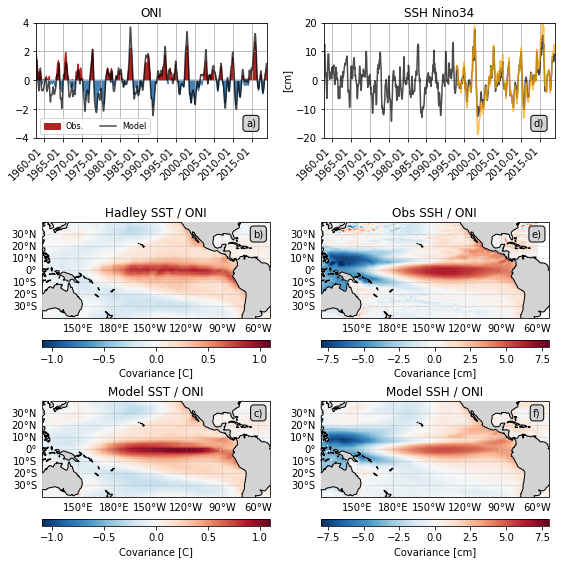
\includegraphics[scale=0.6]{figs/fig1.png}
	\caption{Time evolution of the ONI index in observations and model over the 1958-2018 period (a). ENSO-related SST patterns for observations \citep{raynerGlobalAnalysesSea2003} (b) and model (c) derived from covariance maps of detrended monthly SST anomalies onto the ONI index. Time evolution of zonal current anomalies over the Niño34 region for observations \citep{rioGOCEOceanCirculation2014} and model (d). ENSO-related sea-level and ocean current patterns for observations (e) and model (f) derived from covariance maps of detrended monthly sea-level and current anomalies onto the ONI index. The dashed box represents the Niño34 region used in the averaging.}
	\label{fig:nemo-had-sst}
\end{figure}

Fig.\ref{fig:nemo-had-sst}b and Fig.\ref{fig:nemo-had-sst}c further show the typical SST patterns associated with ENSO for both observations (HadISST1, \citealp{raynerGlobalAnalysesSea2003}) and model by displaying the covariance maps of detrended monthly SST anomalies onto the ONI index. Observed and modelled SST patterns closely resemble each other and are characterized by warm SST anomalies (1\degree{}C) centred in the central and eastern equatorial Pacific  flanked by the traditional horseshoe cooling pattern in the western Pacific extending towards the subtropical north and south Pacific.    


ENSO-driven SST variations are known to be strongly related to ocean current and sea level variations (a proxy for the thermocline depth), with SST signals largely driven by vertical displacement of the equatorial thermocline in response to equatorial wind variations. Figure \ref{fig:nemo-had-sst}d shows the temporal evolution of zonal current anomalies averaged over the Niño34 region for both observations\footnote{\url{https://doi.org/10.48670/moi-00050}} (\citealp{rioGOCEOceanCirculation2014}, available from 1993 to present) and the model, which fairly reproduces the observed anomalies (correlation of 0.89).
%from the DUACS multi-mission altimeter data \footnote{\url{https://doi.org/10.48670/moi-00148}}. The temporal evolution of observed sea level anomalies matches very well the observed SST evolution over the same region (Fig \ref{fig:nemo-had-sst}a), both being correlated at ?.??: the deepening of the thermocline observed in the central and eastern Pacific during El Niño events in response to westerly wind anomalies indeed contribute to El Niño warming by limiting the amount of cold waters brought to the surface, the opposite occurring during La Niña events.  The model accurately reproduces the observed sea level evolution (Fig \ref{fig:nemo-had-sst}d), with a correlation coefficient reaching 0.94 (significant at the $95\%$ level of confidence). 
In addition, the spatial pattern of observed\footnote{\url{https://doi.org/10.48670/moi-00148}} sea-level anomalies associated with ENSO (Fig\ref{fig:nemo-had-sst}e) is characterized by a shallowing of the thermocline  in the western Pacific (negative sea level anomalies) and a deepening of the thermocline  in the central and eastern Pacific (positive sea level anomalies), which is physically consistent with the cooling observed in the west and the warming in the east (Fig\ref{fig:nemo-had-sst}b). As shown on Fig\ref{fig:nemo-had-sst}f, the model captures this zonal sea-level seasaw very accurately.

\subsection{Biogeochemical response}

We then evaluate in Fig\ref{fig:nemo-had-sst}a-c the ability of our simulation to capture cholorophyll variability associated with ENSO variations, which is a proxy for the concentration of low-trophic level organisms that are at the base of the marine food chain. For that purpose, we compare the simulated chlorophyll with observation-based estimates derived from the multi-satellite monthly OceanColour-CCI V5 CHL-a dataset\footnote{\url{http://dx.doi.org/10.5285/1dbe7a109c0244aaad713e078fd3059a}} \citep{sathyendranathOceanColourTimeSeries2019} available over the 1997-09/2018-12 period. This high resolution (4 km)  dataset is regridded on a regular $1\times 1$ grid by computing weighted chlorophyll averages over $24\times24$ boxes, with the weights being provided by the cosine of latitude. When more than $1/3$ of the data used in the averaging is missing, the regridded cell is masked.

\begin{figure}[h!tp]
	\centering
	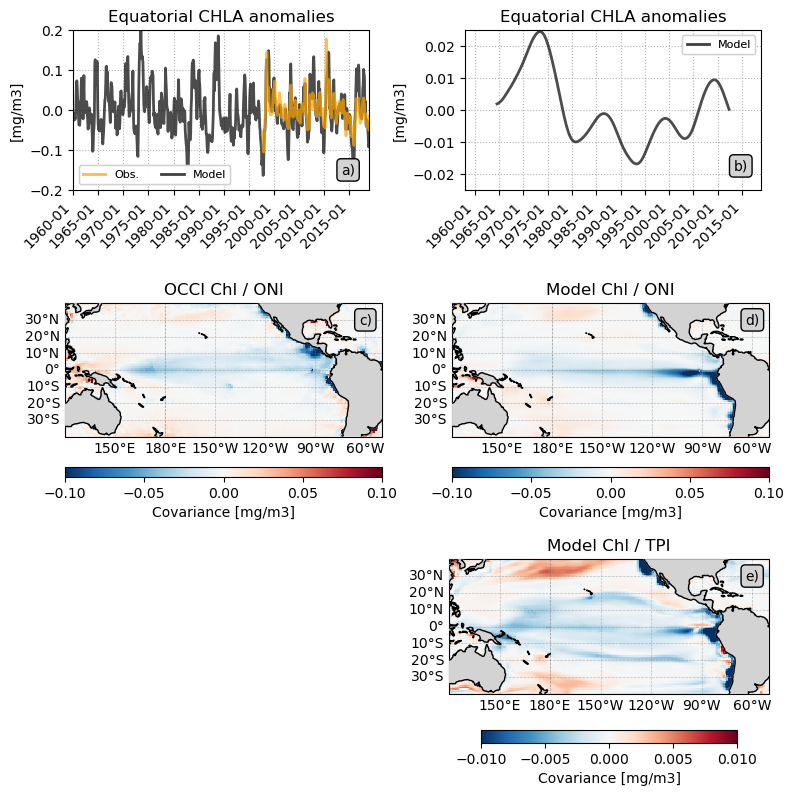
\includegraphics[scale=0.4]{figs/fig2.png}
	\caption{Simulated (black) and observed (yellow) equatorial chlorophyll anomalies (a). Covariance between the chlorophyll anomalies and the ONI index for observations (b) and the model (c). The dashed box represents the equatorial region used in the averaging.}
	\label{fig:nemo-sat-chl}
\end{figure}

Fig \ref{fig:nemo-sat-chl}a shows the temporal evolution of the chlorophyll anomalies averaged in the equatorial Pacific for the model and observations. As already been widely discussed in the literature, El Niño events are associated with a decrease in chlorophyll all along the equator through the combined action of the nutricline deepening in the eastern Pacific and eastward advection of nutrient‐poor waters by anomalous eastward currents in the western and central Pacific. The reverse occurs during major La Niña events. As a result, equatorial chlorophyll anomalies are strongly correlated with Niño34 SST (R=-0.74) and sea-level (R=-0.78) variations. The model accurately reproduces these observed chlorophyll variations, with a correlation coefficient reaching $0.80$ (significant at the $95\%$ level of significance).

Fig \ref{fig:nemo-sat-chl}bc further shows the typical spatial patterns of surface chlorophyll anomalies associated with ENSO for the observations and the model over their common period. In agreement with \ref{fig:nemo-sat-chl}a, El Nino drives a decrease in chlorophyll concentration along the equator east of 150\degree{}E. Despite an overestimation of the modeled chlorophyll decrease in the eastern Pacific along the equator, the observations (upper panel) and the model (lower panel) show similar patterns. Note that recalculating the simulated spatial pattern over the entire modeled period (1958-2018) does not significantly alter the results (not shown). 

\subsection{Ecosystem response}

In this section, we compare the evolution of the simulated epipelagic biomass to available observations in the equatorial Pacific. As mentioned in the introduction, the largest observational inter-annual dataset covering high trophic level marine organisms in the equatorial Pacific is based on tuna catches. Here we use public domain monthly catch of skipjack and yellowfin tuna by purse seiners provided at 1° and 5° spatial resolution by the Western and Central Pacific Fisheries Commission (WCPFC) and processed by the French National Research Institute for Sustainable Development (IRD)\footnote{\url{https://doi.org/10.5281/zenodo.1164128}}, as described in  \citep{taconetGlobalMonthlyCatch2018}. We first extract skipjack and yellowfin purse-seine catches from the raw input file. We then discard observations with a temporal resolution greater than one month and data for which the geographical coordinates are not referenced in the database. The remaining observations are finally binned onto on a regular $1 \times 1$ grid. The final product consists of monthly maps of tuna catches covering the 1959-2018 period. However, due to the limited spatial coverage of the purse-seine fleets in the early part of the record, we only analyse this dataset from 1985 onwards. We compare the catch observations to the biomass of the epipelagic community integrated from 30cm to 70cm, the typical size range of  skipjack and yellowfin tunas caught by purse seiners in this region. In making this comparison, it should be kept in mind that fishing data do not result from a random sampling of the ocean. They are therefore highly biased estimators of the actual biomass of fish swimming in the ocean that are influenced by both climate variability and the numerous socio-economic factors controlling fishing effort dynamics and distribution. Furthermore, although tuna represent the majority of the epipelagic biomass in this size range in this region, our model does not explicitly simulate specific tuna species but generic oceanic communities such as the epipelagic community we study here.

\begin{figure}[h!tp]
	\centering
	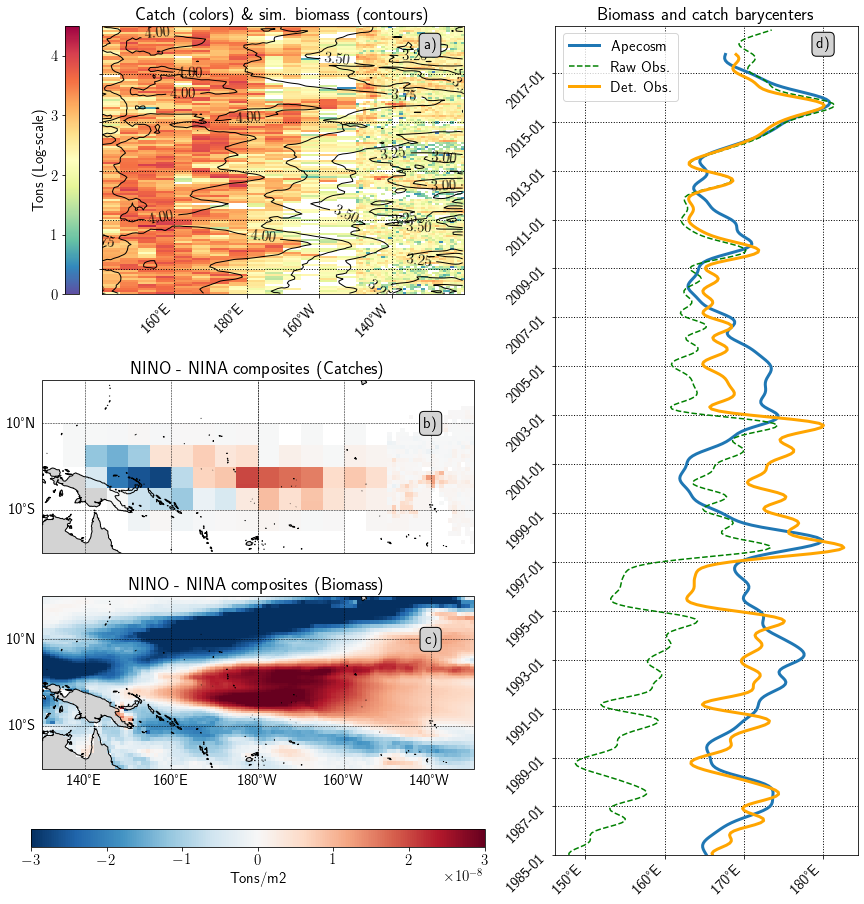
\includegraphics[scale=0.35]{figs/plot_validation_apecosm.png}
	\caption{Time-longitude diagram of observed catches (colors, log-scale in Tons) and simulated epipelagic biomass (contours, log-scale in Tons) integrated between 10N and 10S (a). Catch (b) and simulated fish-biomass (c) difference between El Nino and La Nina composites.}Temporal evolution of the barycenters of simulated epipelagic biomass (black), observed catches (blue) and detrended observed catches (yellow) (d). 
	\label{fig:apecosm_validation}
\end{figure}

Figure \ref{fig:apecosm_validation}a shows the longitude-time diagram of observed catches integrated between 10N and 10S over the period 2008-2018. It highlights significant variations in the zonal extension of tuna catches in the equatorial Pacific. These catches are indeed confined to the west of the dateline during certain periods such as in 2008 and 2011, when La Niña conditions prevail over the Pacific. In contrast, the catch region extends eastward into the central Pacific for other periods such as 2009-2010 and 2014-2016, characterized by El Niño conditions. Despite the different nature of observed catches and our modeled epipelagic biomass, the evolution of the zonal extension of the modeled biomass compares surprisingly well with that of the tuna catches over the recent period: the La Niña events of 2008 and 2011 are indeed characterized by a westward retraction of the epipelagic biomass, while the El Niño periods of 2009-2010 and 2014-2016 are characterized by a clear eastward extension of the epipelagic biomass. Figures \ref{fig:apecosm_validation}b and \ref{fig:apecosm_validation}c show the difference between the observed catches and simulated biomass composites for El Niño (2009-10/2010-03, 2014-10/2015-03, 2015-10/2016-03) and La Niña conditions (2007-10/2008-03, 2008-10/2009-03, 2010-10/2011-03, 2011-10/2012-03). It illustrates the typical east-west shift pattern that is associated with ENSO in the recent period. Observed catches increase in the central and eastern Pacific and decrease in the Western Pacific between La Niña to El Niño conditions, consistent with an eastward shift of the epipelagic biomass. Observed catches and simulated biomass composites show similar patterns, although slightly shifted westward in the model.

To infer whether this agreement holds true over a longer period, Figure \ref{fig:apecosm_validation}d shows the longitude of the observed tuna catch and the modeled biomass barycenters over the period 1985-2018. Consistently with the good agreement between model and observations presented in Fig\ref{fig:apecosm_validation}a, the evolution of model and observations barycenters matches quite well over most of the period considered (2008-2018), with a correlation of 0.68 between the two time series: this is notably the case for the 2014-2016 El Niño sequence, where both model and observations indicate a barycenter eastward shift from 160°E in early 2014 to 180°W in early 2016, before retracting westward after that date. Looking at the observations over the entire observational record, the most striking feature is a gradual eastward shift in the location of the catches barycenter from 155°E in the 80s to 170°E in the last decade. This trend is probably due to the increased power of fishing vessels, which allows them to move further away from their home ports, mostly located in the western Pacific. In addition to this low-frequency eastward trend, higher frequency variations are also evident, especially during the 1986/87, 1997/98 or 2001/02 El Niño events, where observed catches shift eastwards. In order to remove these effects and perform a fair comparison with the model outputs, we smoothed and detrended the time series of the observed catch barycenter longitude (yellow curve on Figure \ref{fig:apecosm_validation}b). The model and detrended observational time series show a reasonable match over the entire time period, with a correlation of 0.45. Their relationship with ENSO is demonstrated by the strong correlation coefficient existing between ONI timeseries and model biomass barycenter (0.74) as well as observed catches barycenter (0.52). While both data and model generally show a westward shift during La Niña conditions and an eastward shift during El Niño conditions, both time series deviate from this general pattern during specific periods, such as the strong La Niña of 1999/2000, which is characterized by a stronger westward retraction in the model or during the warm years of 2003-2005 with the barycenter of observed catches shifting westward relative to that of the modeled biomass.

Overall, the evaluations presented above illustrate the ability of the various model components used here to accurately reproduce the physical, biogeochemical and ecosystem response to ENSO. More specifically, the ecosystem model simulate zonal migrations of large epipelagic communities in the equatorial Pacific in response to ENSO in a manner very similar to that observed for tuna catches. This favourable comparison indicates that our ecosystem simulation is relevant to investigate the processes responsible for the epipelagic community response to ENSO. In what follows, the results are detailed for three selected size classes: 3 cm, representing small epipelagic fishes, 20 cm, representing intermediate sizes, and 90 cm, representing large individuals. The latter two are representative of the lower and upper limits of the size range of tuna exploited by purse seiners in the region (\warn{REF}).

\clearpage